\chapter{Structure du code}

\section{Organisation des classes}
Maintenant que les besoins ont étés traîtés, il convient de s'intéresser à la façon dont nous allons organiser notre code. 
Puisque nous avons choisi Java comme langage de programmation, la conception du programme se fera sous la lumière de la programmation orientée objet. 
Il faut donc définir les classes qui seront utilisées dans le projet.

\paragraph{Le Rubik's cube} Premièrement, notre programme manipule un Rubik's cube. 
Il s'agit donc de définir l'organisation de ces objets:

\begin{figure}[h]
\begin{center}
      \makebox[\textwidth]{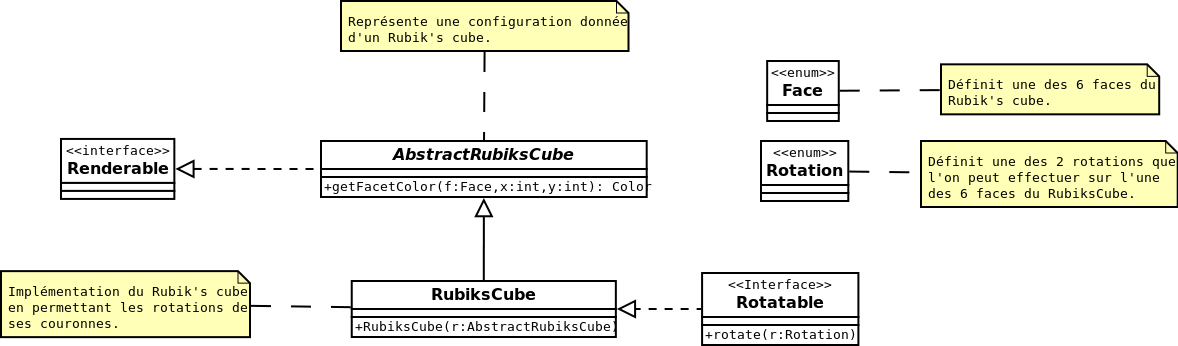
\includegraphics[width=.8\paperwidth]{diagrammes/rubikscube.png}}
\end{center}
    \caption{Diagramme des classes modélisant le Rubik's Cube}
\end{figure}

Ainsi \textit{AbstractRubiksCube} servira lorsque que nous aurons besoin d'informations sur une configuration donnée du Rubik's Cube alors que \textit{RubiksCube} permettra la manipulation de cet objet via l'interface \textit{Rotatable}. 


\paragraph{Rubik'Int} Notre application - donc notre classe principale - sera appelée RubikInt. Elle aura pour rôle de commander les autres objets pour que le programme ait le comportement désiré. Ainsi on peut dessiner un diagramme montrant ses interactions avec les différents autres objets (voir ci-dessous).

\begin{figure}[H]
\begin{center}
      \makebox[\textwidth]{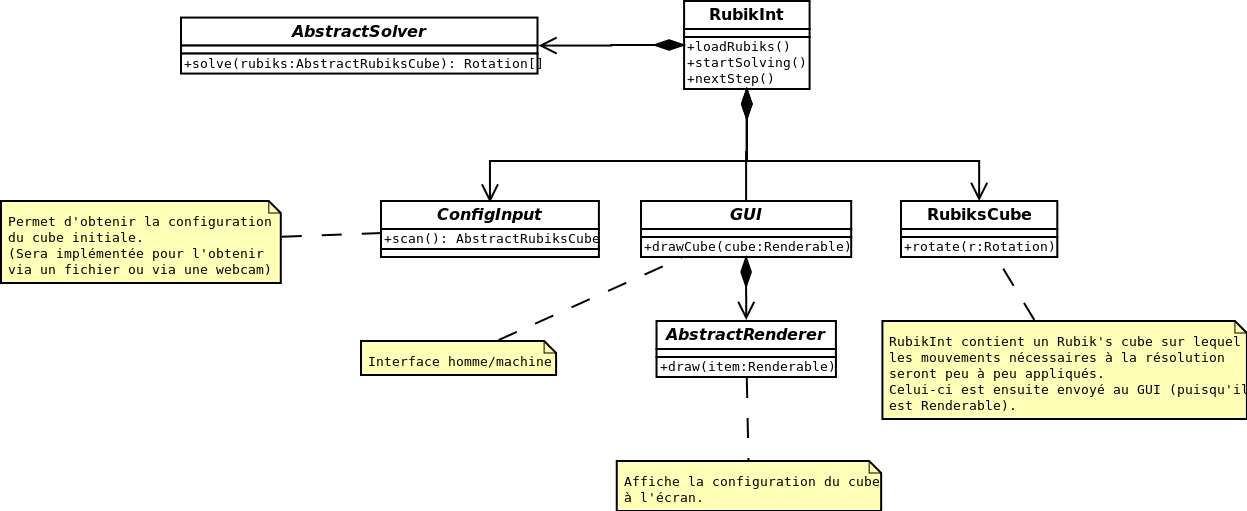
\includegraphics[width=.8\paperwidth]{diagrammes/projet.png}}
\end{center}
    \caption{Diagramme des classes du projet}
\end{figure}

On voit sur le diagramme les différents point importants de notre projet. 
\begin{itemize}
    \item L'interface homme/machine, qui se caractérise par l'implémentation de des classes filles de \textit{GUI} et \textit{AbstractRenderer}.
    \item L'algorithme de résolution qui devra être mis en place dans l'implémentation de la classe fille de \textit{AbstractSolver}. Plusieurs variantes pourront êtres mises en oeuvre.
    \item La structure de donnée choisie pour représenter le Rubik's Cube, dans sa classe \textit{RubiksCube}.
    \item L'interface permettant de rentrer la configuration d'un Rubik's Cube dans \textit{ConfigInput}. Nous pourrons par exemple charger cette configuration d'un fichier, laisser l'utilisateur la rentrer sur une interface graphique ou même l'obtenir via une caméra.
\end{itemize}

\section{Algorithmes de résolution utilisés}
 Résoudre le Rubik's Cube se présente comme une difficulté algorithmique, plusieurs méthodes sont envisagées:
 \begin{itemize}
     \item La première consiste à implémenter un algorithme de résolution simple: par exemple le premier algorithme généralement appris par les humains.\cite{cite2} 
           Le principe de celui-ci est d'envisager la résolution dans l'ordre suivant: d'abord une face, puis la première couronne, la seconde couronne et enfin la dernière face\cite{cite2}. 
           Pour résoudre le Rubik's Cube de cette manière, le programme devra être capable de reconnaître la configuration dans laquelle se trouve le cube à un moment donné et lui appliquer une procédure, c'est-à-dire une suite prédéfinie de rotations. 
           Les autres méthodes utilisées par les humains reposent sur ce même principe avec différentes configurations et procédures. 
           Dans le cas des méthodes dites avancées, c'est-à-dire permettant de résoudre le Rubik's Cube  en un plus petit nombre de rotations, le nombre de configurations et de procédures à apprendre augmente drastiquement.
    \item Un algorithme reposant sur une machine de Boltzmann\cite{cite10} est également envisagée. Cet algorithme aurait une fonction d'évaluation de    l'énergie du cube (plus le cube est proche de sa résolution, plus son énergie est faible) et chercherait à minimiser cette énergie via des rotations  aléatoires ou des procédures aléatoires. Ces procédures auraient d'autant plus de chances d'être choisie que leur action réduit l'énergie du cube.    Cet algorithme pourrait être utilisé conjointement avec le premier pour la résolution.
    \item Un troisième algorithme dit en deux phases consiste à utiliser un algorithme A*\cite{cite3} (parcours d'un arbre en profondeur amélioré par     une heuristique) pour placer les angles du cube au bon endroit lors de la première phase. La seconde phase consiste à utiliser réduire le nombre des  rotations possibles à un groupe de cardinal plus petit.\footnote{Plus d'information sur les groupes du cube \cite{cite12}} Cet algorithme permet de   résoudre le Rubik's Cube en une vingtaine de
        coups, mais est également plus dur à implémenter\cite{cite0}. Cet algorithme est une amélioration d'un algorithme passant par 5 groupes\cite{cite4}.
 \end{itemize}

